\section{Einleitung}
\subsection{Motivation}
\offen{1.1 Motivation -- Stichpunkte im Entwurf}

\subsection{Problemstellung}
\offen{1.2 Problemstellung -- Stichpunkte im Entwurf}

\subsection{Forschungsfragen und Hypothesen}
% abgesegnet am 27.10.2026
\textbf{Zentrale Forschungsfrage:} Kann ein LLM-Agent für einen Geschäftsprozess die geltenden Vorschriften selbst recherchieren, den Arbeitsschritten zuordnen und fehlende Schritte erkennen -- und lassen sich diese Vorschriften in Prüfregeln übersetzen, die das Verhalten eines KI-Agenten zur Laufzeit kontrollieren?

Die zentrale Forschungsfrage wird entlang einer Kette von fünf Schritten untersucht (Abbildung~\ref{fig:untersuchungskette}). Jeder Schritt verarbeitet das Ergebnis des vorherigen und wird durch eine eigene Hypothese geprüft. Ob die Kette als Ganzes trägt, prüft Hypothese H4.

\begin{figure}[H]
  \centering
  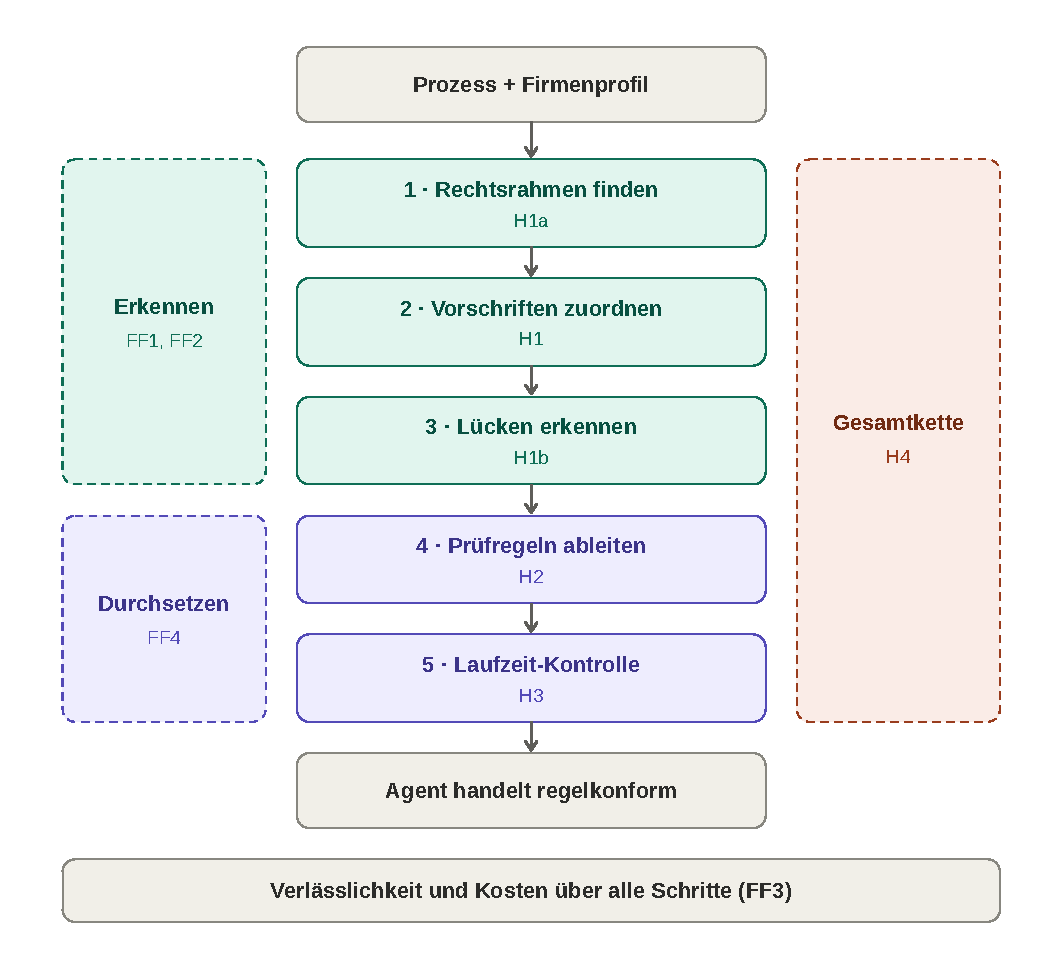
\includegraphics[width=0.85\textwidth]{figures/abb_1_1_untersuchungskette.pdf}
  \caption[Untersuchungskette der Arbeit]{Untersuchungskette der Arbeit. Die Schritte 1 bis 3 erkennen regulatorische Anforderungen, die Schritte 4 und 5 setzen sie zur Laufzeit durch.}
  \label{fig:untersuchungskette}
\end{figure}

\begin{description}[leftmargin=1.2cm,style=nextline]
  \item[FF1] Wie vollständig und wie genau bestimmt ein LLM-Agent mit eigener Recherche die für einen Geschäftsprozess geltenden Regelwerke und ordnet deren Vorschriften den einzelnen Arbeitsschritten zu?
  \begin{description}[leftmargin=1.2cm]
    \item[H1a] Der Agent bestimmt die geltenden Regelwerke nahezu vollständig (\fb{trefferquote} $\geq 0{,}9$).
    \item[H1] Der Agent ordnet die geltenden Vorschriften den Arbeitsschritten mindestens so vollständig zu wie GPT-4 bei Sai et al.~\cite{sai2024} auf Task-Ebene (\fb{trefferquote} $\geq 0{,}62$).
  \end{description}
  \item[FF2] Erkennt der Agent rechtlich gebotene Schritte, die im Prozess fehlen?
  \begin{description}[leftmargin=1.2cm]
    \item[H1b] Der Agent erkennt die Mehrheit der fehlenden Schritte, ohne vorhandene Schritte als fehlend zu melden.
  \end{description}
  \item[FF3] Wie beeinflussen die Gestaltung des Prompts und das Recherchewerkzeug die Vollständigkeit, die Genauigkeit, den Anteil erfundener Normen und die Kosten?
  \item[FF4] Lassen sich die zugeordneten Vorschriften in maschinell prüfbare Regeln übersetzen, mit denen sich das Verhalten eines KI-Agenten zur Laufzeit kontrollieren lässt?
  \begin{description}[leftmargin=1.2cm]
    \item[H2] Aus den zugeordneten Vorschriften lassen sich Prüfregeln erzeugen, die bei Referenzfällen dieselbe Entscheidung treffen wie eine fachliche Prüfung.
    \item[H3] Ein Laufzeitmonitor mit diesen Prüfregeln verhindert unzulässige Aktionen eines KI-Agenten, ohne zulässige Aktionen zu blockieren.
    \item[H4] Auch wenn die Ergebnisse des Agenten aus H1 und H1b unkorrigiert weitergegeben werden, verhindert die Laufzeit-Kontrolle die Mehrheit der unzulässigen Aktionen.
  \end{description}
\end{description}

\subsection{Beitrag der Arbeit}
\offen{1.4 Beitrag}

\subsection{Aufbau der Arbeit}
\offen{1.5 Aufbau -- wird zuletzt geschrieben}
